\documentclass[11pt]{article}
\usepackage[utf8]{inputenc}

\usepackage{hyperref}


\usepackage{amsthm}
\newtheorem{lemma}{Lemma}
\newtheorem{thm}{Theorem}
\newtheorem{conj}{Conjecture}
\newtheorem{prop}{Proposition}

\theoremstyle{definition}
\newtheorem{defn}{Definition}
\newtheorem{example}{Example}
\newtheorem{question}{Question}

\theoremstyle{remark}
\newtheorem{remark}{Remark}

\newcommand{\N}{\ensuremath{\mathbb{N}}}
\newcommand{\Z}{\ensuremath{\mathbb{Z}}}

\usepackage{graphicx}
\usepackage{amsfonts, amsmath}
\usepackage{enumitem}
\usepackage{xcolor}
\usepackage{cleveref}

\usepackage{geometry}
\geometry{margin=1in}

\usepackage{titlesec}
\titleformat*{\section}{\large\bfseries}
\titleformat*{\subsection}{\normalsize\bfseries}

\title{Quantifying and Characterizing Information Loss in Weighted Hypergraph Line Graphs}

\author{Sinan Aksoy, Elie Alhajjar, Jai Aslam, Brianna Chrisman, Sarah Days-Merrill,\\
Helen Jenne, Yosuke Mizutani, Tracey Oellerich, and Ethan Semrad}

\date{\today}



\begin{document}

\maketitle

\section{Introduction}

\section{Gram mates}

\begin{defn}\cite[Definition 2.1]{Kirkland}
Two $(0, 1)$ matrices $A$ and $B$ are Gram mates and $A$ is called a Gram mate to $B$ if $AA^{T} = BB^{T}$, $A^{T}A = B^{T}B$, and $A \neq B$. 
\end{defn}

Kim and Kirkland study Gram mates of the form $(A, A+E)$, where $E$ is matrix containing 0's, 1's and $-1$'s whose row and column sums are 0. When $A$ and $A+E$ are Gram mates, $E$ is said to be {\em realizable} (with respect to Gram mates). 

In their paper, Kim and Kirkland completely characterize Gram mates of the form $(A, A+E)$ in the cases where $E$ has rank 1 or 2. In the rank 1 case, they prove the following theorem. 

\begin{thm} 
\label{thm:thm47}
Suppose that $E$ is a realizable matrix of rank 1:
\[
E = \begin{pmatrix}
J_{k_{1}, k_{2}} & -J_{k_{1}, k_{2}} & 0 \\
-J_{k_{1}, k_{2}} & J_{k_{1}, k_{2}} & 0 \\
0 & 0 & 0
\end{pmatrix}
\]
for some $k_1, k_2 > 0$. Here, $J_{k_{1}, k_{2}}$ is the all ones matrix with dimensions $k_1 \times k_2$. Let
\[
A = \begin{pmatrix}
0 & J_{k_{1}, k_{2}} & X_{1} \\
J_{k_{1}, k_{2}} & 0 & X_{2} \\
X_{3} & X_{4} & Y
\end{pmatrix}
\]
be a $(0, 1)$ matrix compatible with the partition of $E$. Then, we have the following:
\begin{itemize}
\item[(i)] $A$ and $A+E$ are Gram mates if and only if ${\bf 1}^{T} X_{1} = {\bf 1}^{T} X_{2}$ and $X_{3}{\bf 1} = X_{4}{\bf 1} $
\item[(ii)] $E$ is realizable
\item[(iii)] For any Gram mates via $E$, they are convertible via each other. 
\item[(iv)] For any Gram mates via $E$, their Gram singular value is $\sqrt{k_1 k_2}$, and the corresponding left and right singular vectors are (up to sign) 
$\dfrac{1}{\sqrt{2k_1}}
\begin{pmatrix}
 -{\bf 1}_{k_{1}}  \\
 {\bf 1}_{k_{1}} \\
 0 
 \end{pmatrix}$ and 
 $\dfrac{1}{\sqrt{2k_2}}
\begin{pmatrix}
 -{\bf 1}_{k_{2}}  \\
 {\bf 1}_{k_{2}} \\
 0 
 \end{pmatrix}$, respectively. 
\end{itemize}

\end{thm}

\begin{remark}
Note that Theorem~\ref{thm:thm47} does not guarantee that $A$ and $A+E$ are not isomorphic. (Two matrices $A$ and $B$ are isomorphic if there exist permutation matrices $P$ and $Q$ such that $A = PBQ$.)
\end{remark}


\begin{question}
Can we interpret the differences between $A$ and $A+E$ in the context of the hypergraph? That is, can we come up with a sequence of local moves that transforms the hypergraph with incidence matrix $A$ to the hypergraph with incidence matrix $A+E$?
\end{question} 

\begin{question}
Can we come up with an algorithm to determine whether an incidence matrix of a hypergraph of real data can be written as a matrix of the form $A$ from Theorem~\ref{thm:thm47}? 
\end{question}

\begin{question}
We know from Kirkland (2017) \cite{kirkland2017} that there are gram mates that are $k$-uniform hypergraphs. Are those gram mates of the form given in Theorem~\ref{thm:thm47}? If not, are there $k$-uniform gram mates of the form $(A, A+E)$, where $A$ and $E$ are as described in Theorem~\ref{thm:thm47}?
\end{question} 

Using this theorem, we get the following example. 

\begin{example}\cite[Example 4.9]{Kirkland}
Let
$$A = 
\begin{pmatrix}
0 & 0 & 1 & 1 & 1 & 1 & 0 \\
0 & 0 & 1 & 1 & 0 & 0 & 1 \\ \hline
1 & 1 & 0 & 0 & 1 & 1 & 1 \\
1 & 1 & 0 & 0 & 0 & 0 & 0 \\ \hline
1 & 0 & 1 & 0 & 1 & 1 & 1 \\
1 & 0 & 1 & 0 & 1 & 1 & 1 \\
0 & 1 & 1 & 0 & 1 & 1 & 1 \\
\end{pmatrix}, E = 
\begin{pmatrix}
1 & 1 & -1 & -1 & 0 & 0 & 0 \\
1 & 1 & -1 & -1 & 0 & 0 & 0 \\ \hline
-1 & -1 & 1 & 1 & 0 & 0 & 0 \\
-1 & -1 & 1 & 1 & 0 & 0 & 0 \\ \hline
0 & 0 & 0 & 0 & 0 & 0 & 0 \\
0 & 0 & 0 & 0 & 0 & 0 & 0 \\
0 & 0 & 0 & 0 & 0 & 0 & 0 \\
\end{pmatrix}, 
$$
Then 
$$B = \begin{pmatrix}
1 & 1 & 0 & 0 & 1 & 1 & 0 \\
1 & 1 & 0 & 0 & 0 & 0 & 1 \\ \hline
0 & 0 & 1 &1 & 1 & 1 & 1 \\
0 & 0 & 1 & 1 & 0 & 0 & 0 \\ \hline
1 & 0 & 1 & 0 & 1 & 1 & 1 \\
1 & 0 & 1 & 0 & 1 & 1 & 1 \\
0 & 1 & 1 & 0 & 1 & 1 & 1 \\
\end{pmatrix}$$



{\bf to do:} add vertical lines to this matrix to show the blocks more clearly

The hypergraphs with incidence matrices $A$ and $B$ are shown below:

\begin{center}
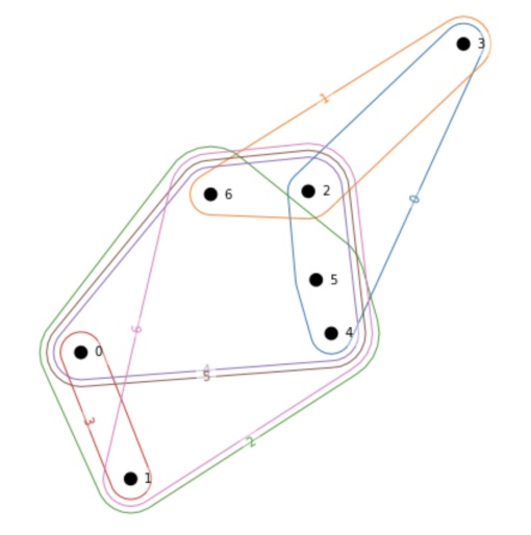
\includegraphics[width=2in]{./images/7by7ex_A}
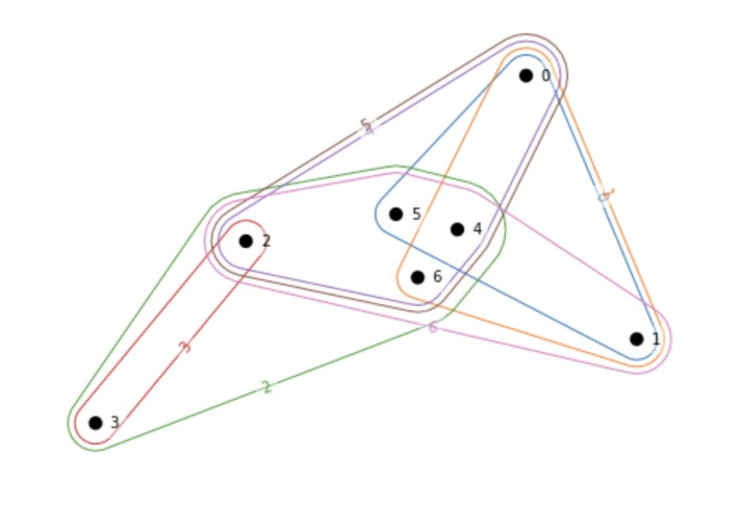
\includegraphics[width=3in]{./images/7by7ex_B}
\end{center}


$A$ and $B$ are not isomorphic. A (very preliminary) investigation showed several different structural properties between $A$ and $B$ when considered as bipartite graphs (so the matrices $A$ and $B$ are taken to be bipartite adjacency matrices. Namely, when $A$ and $B$ are bipartite adjacency matrices, the corresponding bipartite graphs have different $k$-core, different diameter, and differently sized maximal independent sets. Below we show the 2-core and 3-core of the bipartite graph with adjacency matrix $A$. This graph has no 4-core.
\begin{center}
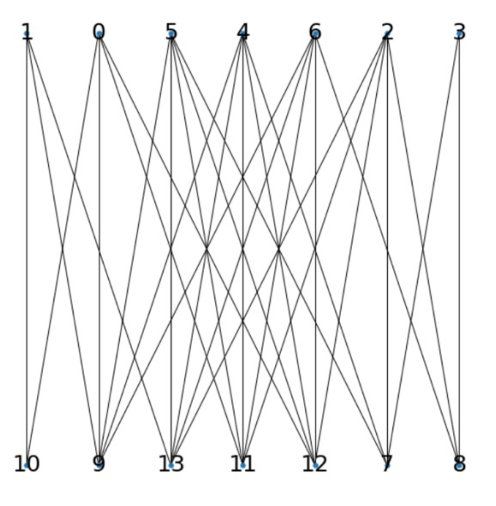
\includegraphics[width=1.9in]{./images/2coreA}
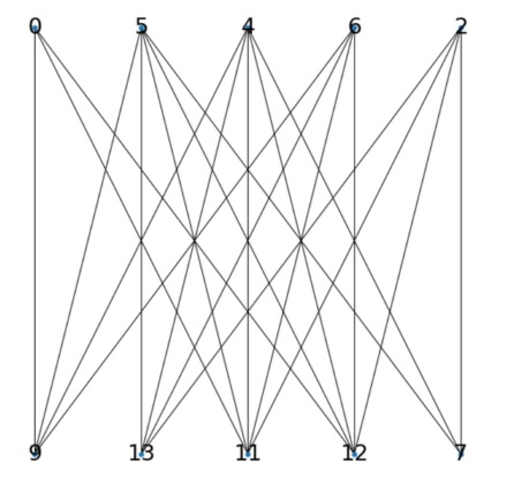
\includegraphics[width=2in]{./images/3coreA}
\end{center}

On the other hand, the bipartite graph with adjacency matrix $B$ has the 2-core, 3-core and 4-core shown below. 

\begin{center}
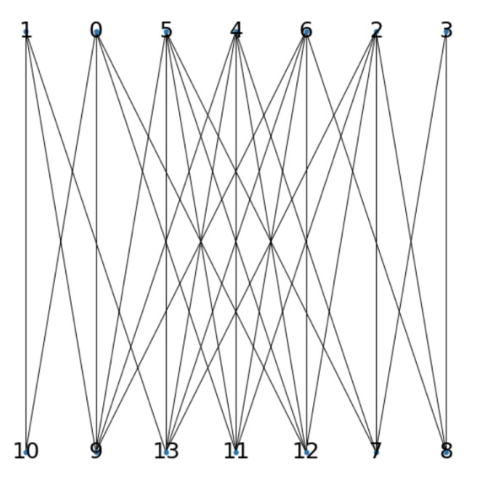
\includegraphics[width=2in]{./images/2coreB}
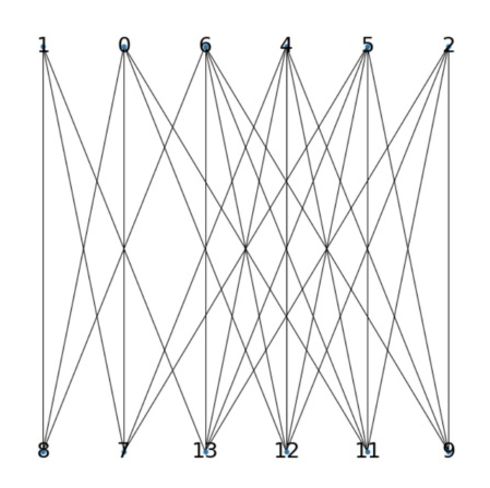
\includegraphics[width=2in]{./images/3coreB}
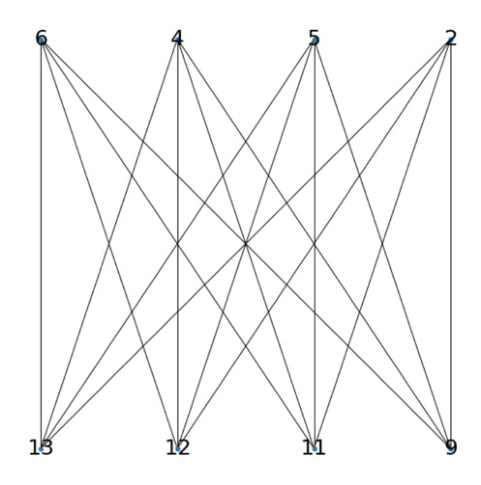
\includegraphics[width=2in]{./images/4coreB}
\end{center}


The bipartite graph with adjacency matrix $A$ has diameter 5, while the bipartite graph with adjacency matrix $B$ has diameter 4. After looking at the graphs in more detail, the bipartite graph with adjacency matrix $A$ had one path of length 5: from vertex 3 to vertex 10. After adding $E$, these two vertices are adjacent, and no longer paths are created. So the bipartite graph corresponding to $A+ E$ has diameter 4. 





           		

\end{example}

\begin{question}
What other structural differences are there between the gram mates in this example?
\end{question}

\begin{question}
Can we generalize this example to find a class of gram mates that all have a different $k$-core?
Can we generalize this example to produce two gram mates where one has bipartite diameter $d$ and the other has e smaller bipartie diameter (or even much smaller?)
\end{question}


While Theorem 4.7 doesn't guarantee that the two gram mates $(A, A+E)$ will be non-isomorphic, in Section 6, Kim and Kirkland give conditions under which we can be assured that $A$ is not isomorphic to $A+E$. The condition that needs to be checked (the matrix $Y$ is ``fixable'') is not completely easy to understand. 

\begin{remark}
After understanding the condition on $Y$ in Theorem 6.10 we can use this theorem to generate all examples of non-isomorphic gram mates of a given size, which may be helpful to identify structural differences. 
\end{remark}

\begin{question}
Can we find gram mates that are not of the form $(A, A+E)$? 
{\bf add citation, either kirkland or everett and borgatti} points out that gram mates can be constructed with the following procedure. Let $D$ be a diagonal matrix with positive values on the diagonal. Let $P$ be an orthogonal mattrix of the same size as $D$. Let $\tilde{D}$ be $D$ with any number of diagonal values made negative. 
 $A = PDP^{T}$ and $B = P\widetilde{D}P^{T}$ are non-isomorphic. If $A$ and $B$ are both $(0, 1)$ matrices, we have gram mates.
\end{question}

\begin{question}
How do we check if a hypergraph from real data has a gram mate?
\end{question}
\section{Everett and Borgatti}

Everett and Borgatti \cite{Everett} give an algorithm to recover $A$ given $AA^{T}$ and $A^{T}A$.

The idea of the algorithm is to use the singular value decomposition of $A$. SVD says that $A$ can be written as $A = U \Sigma V^{T}$, where 
$U = \begin{pmatrix}
{\bf u_{1}} & {\bf u_{2}} & \cdots & {\bf u_{m}} \\
\end{pmatrix}$ and $V = \begin{pmatrix}
{\bf v_{1}} & {\bf v_{2}} & \cdots & {\bf v_{n}} \\
\end{pmatrix}$ are the matrices consisting of the eigenvectors of $AA^{T}$ and $A^{T}A$, respectively. $\Sigma$ is a diagonal matrix with the positive square roots of the eigenvalues of $AA^{T}$ on the diagonal. These eigenvectors are not unique, so we require that the eigenvectors have unit norm. Also, we need to assume that $AA^{T}$ has unique eigenvectors. 

The algorithm is as follows. \\

\noindent Given $C = AA^{T}$ and $L = A^{T}A$:

	Compute the eigenvectors of $C$ (this gives the matrix $U$)
	
	Compute the eigenvectors of $L$ (this gives the matrix $V$)
	
	Compute the eigenvalues of $C$ and construct the diagonal matrix $\Sigma$ whose entries are the positive square roots of the eigenvalues of $C$.
	
	(Note about implementation: if you use scipy or numpy to compute the eigenvectors of $C$ (and $L$), then you have to take care to sort the eigenvalues so that they are in descending order, and then reorder the columns of $U$ (and $V$) as needed. 
	
	Compute $R = U \Sigma V^{T}$. If $R$ is a binary matrix, return $R$. 
	
	Otherwise, for all pairs $(I, J)$ in $\mathcal{P}(\{1, 2, \ldots m \}) \times \mathcal{P}(\{1, 2, \ldots n \})$: (where $\mathcal{P}(\{1, 2, \ldots m \})$ denotes the power set of $\{1, 2, \ldots m \}$) 
	
\hspace{10pt}	Let $\widetilde{U}$ be the matrix $U$ except the columns with indices $I$ have opposite sign.
	
\hspace{10pt}		Let $\widetilde{V}$ be the matrix $V$ except the columns with indices $J$ have opposite sign.
	
\hspace{10pt}	Compute $R = \widetilde{U} \Sigma \widetilde{V}^{T}$. If $R$ is a binary matrix, return $R$ and terminate the algorithm. 

{\bf to do:} fix the formatting of the algorithm to make it more readable. 
	
\begin{remark}
We checked that this algorithm works on all binary $m \times n$ matrices with $m \leq 4$ and $n \leq 5$. Additionally, we checked it on a couple Erdos-Renyi hypergraphs (size $10 \times 15$). Haven't determined yet how large we can make the hypegraphs before it starts to slow down. 
\end{remark}
	
\begin{remark}
I think we can modify this algorithm so that, given a matrix $A$, we can find all Gram mates of $A$. The modification is to compute $AA^{T}$ and $A^{T}A$ and instead of terminating the algorithm when we find a binary matrix, return all binary matrices that are not equal to $A$ (or perhaps all binary matrices that are not isomorphic to $A$). This will be very slow!
\end{remark}

\begin{question}
Are there Gram mates with equivalence classes of size larger than 2?
\end{question}

\begin{question}
Can we make this more efficient? (by cutting down on the subsets that we're checking)
\end{question}

\begin{question}
Everett and Borgatti say that if the reconstructed matrix from the algorithm is binary ``with very high probability it will be either $A$ or a matrix that is isomorphic to $A$''. Can we formalize and prove this statement? Or has this already been done by Kirkland in 2017 -- he has some kind of result about the measure of the rarity of Gram mates. 
\end{question}

\begin{question}
Is the $7 \times 7$ example in Kim and Kirkland \cite{Kirkland} the smallest gram mate?
\end{question}

\section{Hardness Results}

We consider several variants of the Boolean matrix factorization problem:
 given a symmetric square matrix $B \in \Z^{n \times n}$, find $A \in \{0,1\}^{n \times m}$ such that $B=AA^T$ or similar conditions.
We here use Feldmann et al.'s notation \cite{feldmann_fixed-parameter_2020}.
%
We allow matrices to have wildcard entries in the diagonal that will be denoted by $\star$.
We define $\Z^\star := \Z_{\geq 0} \cup \{\star\}$.
For $x, y \in \Z$, we write $x \stackrel{\star}{=} y$ if and only if either $x=y$, or at least one of $x$ and $y$ is $\star$.
For two matrices $X$ and $Y$ in $(\Z^\star)^{m\times n}$, we write $X \stackrel{\star}{=} Y$
 if and only if $X_{i,j} \stackrel{\star}{=} Y_{i,j}$ for all $i$, $j$.
Further, $\|\cdot\|_0$ denotes the number of nonzero entries.
%
\Cref{tab:hardness} summarizes known and newly established hardness results.

\begin{table*}[ht]
  \centering
  \small

  \begin{tabular}{|c|c|p{0.18\textwidth}|p{0.18\textwidth}|p{0.3\textwidth}|p{0.18\textwidth}|}
    \hline
    \#
    &Given
    &\multicolumn{1}{c|}{Given $B$} 
    &\multicolumn{1}{c|}{Find $A$} 
    &\multicolumn{1}{c|}{Problem / Interpretation}
    &\multicolumn{1}{c|}{Hardness}
    \\
    \hline
    (1) & $m \in \N$ & $B \in \{0,1,\star \}^{n \times n}$,\newline $b_{i,i}=\star\quad\forall i$
     & $A \in \{0,1\}^{n \times m}$,\newline $B\stackrel{\star}{=}AA^T$
     & Edge Clique Partition of a graph with $n$ vertices; decompose all edges into a set of $m$ cliques (if such one exists).
     & NP-hard \cite{shaohan1988complexity}\\
    \hline
    (2) & $m \in \N$ & $B \in (\Z^\star)^{n \times n}$,\newline $b_{i,i}=\star \quad\forall i$
     & $A \in \{0,1\}^{n \times m}$,\newline $B\stackrel{\star}{=}AA^T$
     & Weighted Edge Clique Partition of a graph with $n$ vertices
     (equivalently, Edge Clique Partition on a multigraph without loops);
     decompose all weighted edges into a multiset of $m$ cliques.
     & NP-hard \cite{feldmann_fixed-parameter_2020,cooley_parameterized_2021}\\
    \hline
    (3) & $m \in \N$ & $B \in \Z^{n \times n}$
    & $A \in \{0,1\}^{n \times m}$,\newline $B=AA^T$
    & (a) Weighted Clique Decomposition of a hypergraph with $n$ vertices and $m$ hyperedges.
    (b) Recovering a hypergraph with $m$ vertices and $n$ hyperedges from the given weighted line graph.
    & \textcolor{blue}{NP-hard}\\
    \hline
    (4) & --- & $B \in (\Z^\star)^{n \times n}$,\newline $b_{i,i}=\star \quad\forall i$
    & $A \in \{0,1\}^{n \times m}$,\newline $B\stackrel{\star}{=}AA^T$
    & (a) Weighted Clique Decomposition of a hypergraph with $n$ vertices 
    and \textit{any number of} hyperedges, \textbf{ignoring the diagonal entries in $B$ (vertex weights)}.
    (b) Recovering a hypergraph with \textit{any number of} vertices and 
    $n$ hyperedges from the given weighted line graph, ignoring the diagonal entries in $B$.
    & \textcolor{blue}{P}\\
    \hline
    (5) & --- & $B \in \Z^{n \times n}$
    & $A \in \{0,1\}^{n \times m}$,\newline $B=AA^T$
    & (a) Weighted Clique Decomposition of a hypergraph with $n$ vertices and \textit{any number of} hyperedges.
    (b) Recovering a hypergraph with \textit{any number of} vertices and $n$ hyperedges from the given weighted line graph.
    & Open? Literature survey needed.\\
    \hline
    (6) & $k \in \N$ & $B \in \Z^{n \times n}$
    & $A \in \{0,1\}^{n \times m}$,\newline 
    $\|A_{i,*}\|_0=k\quad\forall i$,\newline
    $B=AA^T$
    & (a) Weighted Clique Decomposition of a $k$-\textbf{regular} hypergraph with $n$ vertices.
    (b) Recovering a $k$-\textbf{uniform} hypergraph with $n$ hyperedges from the given weighted line graph.
    & P when $k=2$ \cite{roussopoulos_max_1973,lehot_optimal_1974,syslo_labeling_1982,degiorgi_dynamic_1995,liu_iligra_2015};\newline
    NP-hard when $k \geq 3$ \cite{poljak_complexity_1981,chen_symmetric_2022}\\
    \hline
    (7) & $k \in \N$ & $B \in \Z^{n \times n}$
    & $A \in \{0,1\}^{n \times m}$,\newline 
    $\|A_{*,j}\|_0=k\quad \forall j$,\newline
    $B=AA^T$
    & (a) Weighted Clique Decomposition of a $k$-\textbf{uniform} hypergraph with $n$ vertices.
    (b) Recovering a $k$-\textbf{regular} hypergraph with $n$ hyperedges from the given weighted line graph.
    & Open? Literature survey needed.\\
    \hline
  \end{tabular}

  \caption{%
  Known and established hardness results (new results in blue).
  }
  \label{tab:hardness}
\end{table*}


\begin{thm}\label{thm:hardness-bounded}
  Problem (3) in \Cref{tab:hardness} is NP-hard.
\end{thm}

\begin{proof}[Proof Sketch of Theorem~\ref{thm:hardness-bounded}]
  TODO: Yo
\end{proof}

\begin{thm}\label{thm:hardness-unbounded}
  Problem (4) in \Cref{tab:hardness} can be solved in polynomial time in $n$.
\end{thm}

\begin{proof}[Proof Sketch of Theorem~\ref{thm:hardness-unbounded}]
  Consider this problem as Weighted Clique Decomposition.
  %
  First, observe that adding a clique of size 1 does not change the feasibility
  because the diagonal entries in $B$ are ignored.
  If the instance is feasible, then there must exist a solution without a clique of size 1.
  %
  Therefore, it is enough to construct a set of cliques of size 2 in a greedy manner.
  %
  This construction will require $\sum_{1 \leq i < j \leq n}b_{i,j}$ cliques.
\end{proof}


\section{Software}

%TODO[Yo]

\bibliographystyle{plain}
\bibliography{refs}

\end{document}
